

\subsection{Main Results}
We first establish our baseline by directly prompting frontier LLMs, such as GPT-4.1, Gemini 2.5 Pro, and Claude 3.7 Sonnet, to produce the kernels. As shown in Table\ref{tab:baselines}, across all models, direct prompting yields low execution accuracy and suboptimal performance, indicating that even state-of-the-art LLMs struggle to produce correct and efficient low-level code without further guidance.

Introducing one-shot prompting—where a single example retrieved from TritonBench trainset is provided—consistently improves both call accuracy and execution accuracy compared to zero-shot prompting. In most cases, one-shot prompting also leads to higher speedup, suggesting that the additional context helps LLMs generate more efficient kernels. However, a notable exception is observed with Gemini 2.5 Pro, where one-shot prompting results in lower speedup than direct prompting, despite improvements in accuracy.

Table\ref{tab:baselines} shows the direct prompting results on the ROCm benchmark. Direct prompting with GPT-4.1 fails to generate any valid kernels, underscoring the challenge of targeting non-CUDA platforms. In contrast, Gemini 2.5 Pro achieves better results than GPT-4.1 on both the TritonBench-revised and ROCm benchmarks, though the overall performance remains limited.

As shown in Table\ref{tab:geak_on_tritonbench} and Table\ref{tab:geak_on_rocm_mi300}, compared to direct LLM prompting, our system GEAK delivers significantly stronger results. On MI300, GEAK achieves 54.89\% execution accuracy and a 2.59× speedup on TritonBench-revised Benchmark, and 63.33\% execution accuracy and 0.92x speedup on ROCm Benchmark, demonstrating the effectiveness of our agent framework. We also present a case study in Appendix \ref{appendix:case-study} on $triton\_test\_flip.py$ kernel analyzing potential strategies for performance gain.

\begin{table}
 \caption{Baseline Results}
  \centering
  \begin{threeparttable}
  \begin{tabular}{llll}
    \toprule
    Model     & Call Accuracy (\%)     & Exec Accuracy {\%} & Speedup \\
    \midrule
    \multicolumn{4}{c}{TritonBench-modified benchmark}                   \\
    \midrule
    GPT4.1 & 14.67 / 19.02  &  8.70 / 14.13  & 0.52 / 0.53    \\
    GPT4o     &  10.87 / 14.13  & 7.07 / 9.24 & 0.51 / 0.53      \\
    Gemini2.5pro     & 20.65 / 21.74       & 14.13 / 16.85 & 1.33 / 0.96  \\
    Claude 3.7  & 11.41 / 20.11 & 7.07 / 15.22 & 0.61 / 0.96 \\
    \midrule
    \multicolumn{4}{c}{ROCm benchmark (0-shot results only) } \\
    \midrule
    GPT 4.1 & 0 & 0 & 0 \\
    Gemini-2.5 Pro & 40 & 16.66 & 0.91 \\
    \bottomrule
  \end{tabular}
  \label{tab:baselines}
  \begin{tablenotes}
  \small
\item Note:  numbers to the left of ‘/’ indicate 0-shot results and to the right are 1-shot prompting results.
\end{tablenotes}
  \end{threeparttable}
\end{table}
\begin{table}
 \caption{GEAK on TritonBench-Modified Benchmark }
  \centering
  \begin{threeparttable}
  \begin{tabular}{lllll}
    \toprule
    Difficulty level & Correctly generated kernels & Total kernels in dataset & Exec Accuracy (\%) & Average Speedup  \\
    \midrule
    1 & 2 / 3 & 3 & 66.67 / 100.0 & 1.24 / 1.16 \\
    2 & 23 / 22 & 27 & 85.19 / 81.48 & 4.78 / 1.69 \\
    3 & 39 / 41 & 65 & 60.00 / 63.08 & 1.57 / 3.02 \\
    4 & 32 / 34 & 84 & 38.10 / 40.48 & 2.24 / 2.86 \\
    5 & 1 / 1 & 5 & 20.00 / 20.00 & 0.14 / 0.61 \\
    \midrule
    overall & 97 / 101 & 184 & 52.72 / 54.89 & 2.42 / 2.59 \\
    \bottomrule
  \end{tabular}
  \label{tab:geak_on_tritonbench}
  \begin{tablenotes}
  \small
\item Note:  numbers to the left of ‘/’ indicate results on MI250 and to the right are results on MI300.
\end{tablenotes}
  \end{threeparttable}
\end{table}
\begin{table}
 \caption{GEAK on ROCm Benchmark}
  \centering
  \begin{tabular}{lllll}
    \toprule
    Difficulty level & Correctly generated kernels & Total kernels in dataset & Exec Accuracy (\%) & Average Speedup  \\
    \midrule
    overall & 19 & 30 & 63.33 & 0.92 \\
    \bottomrule
  \end{tabular}
  \label{tab:geak_on_rocm_mi300}
\end{table}

\subsection{Ablation Experiments}

\subsubsection{Sequential Scaling}
We investigate the impact of increasing inference-time compute on accuracy and performance, focusing on the sequential scaling dimension.

The experimental results in Table\ref{tab:sequential_scaling_mi250} indicate that increasing the number of iterations leads to a steady improvement in both the accuracy and performance of GEAK. As the number of iterations increases, we observe a monotonic improvement in both call and execution accuracy, culminating at iter19 with 63.04\% call accuracy and 44.02\% execution accuracy—more than 3× higher than the baseline.

In terms of performance, speedup improves significantly in the early iterations, with iter1 already reaching 1.89×, the highest across all settings. This sharp gain is likely due to early corrections of suboptimal code generations. Although the speedup fluctuates slightly in later iterations, it consistently stays above 1.4× from iter7 onwards, suggesting that continued refinement contributes to runtime efficiency as well.

Notably, iteration count beyond 10 still yields meaningful gains: call accuracy increases from 56.52\% (iter9) to 63.04\% (iter19), and execution accuracy from 40.76\% to 44.02\%. These results validate the effectiveness of iterative refinement in improving both correctness and efficiency.

Overall, the analysis confirms that sequential compute budget is a powerful scaling axis for GEAK, enabling it to progressively refine outputs with improved correctness and performance.

\begin{table}
 \caption{Sequential Scaling of GEAK on TritonBench-Modified Benchmark on MI250}
  \centering
  \begin{tabular}{llll}
    \toprule
    \#iterations & call acc(\%) & exec acc(\%) & speedup  \\
    \midrule
    iter0 & 21.2 & 13.04 & 1.02 \\
    iter1 & 33.15 & 26.63 & \textbf{1.89} \\
    iter2 & 41.85 & 30.98 & 1.69 \\
    iter3 & 47.28 & 34.24 & 1.39 \\
    iter4 & 50.54 & 37.5 & 1.39  \\
    iter5 & 57.61 & 37.5 & 1.63 \\
    iter6 & 50.04 & 37.5 & 1.31 \\
    iter7 & 54.39 & 39.13 & 1.48 \\
    iter8 & 62.5 & 40.22 & 1.67 \\
    iter9 & 56.52 & 40.76 & 1.45 \\
    iter10 & 62.5 & 40.22 & 1.75 \\
    iter11 & 55.43 & 40.76 & 1.45 \\
    iter12 & 57.07 & 42.39 & 1.16 \\
    iter13 & 59.78 & 41.85 & 1.75 \\
    iter14 & 61.41 & 40.76 & 1.76 \\
    iter15 & 57.07 & 43.48 & 1.65 \\
    iter16 & 60.33 & 42.93 & 1.57 \\
    iter17 & 60.87 & 43.48 & 1.85 \\
    iter18 & 61.96 & 43.48 & 1.74 \\
    iter19 & \textbf{63.04} & \textbf{44.02} & 1.55 \\
   
    \bottomrule
  \end{tabular}
  \label{tab:sequential_scaling_mi250}
\end{table}

\subsubsection{Parallel Scaling}
We demonstrate how increasing inference-time compute through parallel scaling improves both accuracy and performance. Specifically, we fix the number of sequential iterations to 10 and explore how varying the number of parallel runs during inference affects the results. Experiments are conducted on both MI250 and MI300 GPUs to ensure the findings generalize across hardware generations.

Figure\ref{fig:fig1} and Figure\ref{fig:fig2} show inference time scaling laws on ROCm and TritonBench-revised benchmarks, respectively. Both call and execution accuracy scale almost log-linearly with respect to the number of parallel runs,

These findings underscore the complementary role of parallel scaling alongside sequential refinement as two orthogonal axes to boost inference quality. Together, they provide a flexible mechanism for tuning the accuracy-performance tradeoff under a given compute budget.

The parallel scaling analysis reveals several critical insights for the GEAK framework's design and implementation strategy. First, parallel scaling provides complementary benefits to sequential refinement, enabling the framework to achieve higher accuracy without proportionally increasing latency. This orthogonal improvement axis allows GEAK to optimize both accuracy and efficiency simultaneously.

The consistent scaling patterns across different hardware platforms demonstrate that GEAK's parallel scaling mechanisms are robust and portable. The framework can leverage available computational resources effectively regardless of the underlying GPU architecture, making it suitable for diverse deployment environments.

The substantial improvements in Call Accuracy relative to Execution Accuracy indicate that parallel scaling particularly benefits high-level reasoning and decision-making processes. This suggests that GEAK's parallel mechanisms are especially valuable for complex inference tasks that require sophisticated logical reasoning rather than simple execution steps.

Finally, the scaling characteristics support GEAK's flexible architecture design, where parallel compute resources can be dynamically allocated based on task complexity and accuracy requirements. This adaptability ensures that the framework can optimize performance across different use cases while maintaining computational efficiency.

\begin{table}
 \caption{TritonBench-Modified Benchmark: GEAK Sequential@10 + Parallel@10 on MI250 - GPT4.1}
  \centering
  \begin{tabular}{lll}
    \toprule
    Pass@K & call acc(\%) & exec acc(\%) \\
       \midrule
    1 & 56.52 & 40.76 \\
    2 & 66.30 & 45.65 \\
    3 & 72.83 & 48.91 \\
    4 & 78.80 & 50.0 \\
    5 & 81.52 & 50.0 \\
    6 & 82.61 & 49.46 \\
    7 & 85.87 & 52.17 \\
    8 & 86.41 & 53.26 \\
    9 & 86.41 & 53.26 \\
   
    \bottomrule
  \end{tabular}
  \label{tab:parallel_scaling_tritonbench_mi250}
\end{table}
\begin{table}
 \caption{TritonBench-Modified Benchmark: GEAK Sequential@10 + Parallel@10 on MI300 - GPT4.1}
  \centering
  \begin{tabular}{lll}
    \toprule
    Pass@K & call acc(\%) & exec acc(\%) \\
       \midrule
    1 & 54.78 & 35.38 \\
    2 & 71.31 & 43.95 \\
    3 & 78.85 & 47.53 \\
    4 & 83.13 & 49.55 \\
    5 & 85.92 & 50.92 \\
    6 & 87.87 & 51.96 \\
    7 & 89.30 & 52.81 \\
    8 & 90.37 & 53.55 \\
    9 & 91.20 & 54.24 \\
    10 & 91.85 & 54.89 \\
   
    \bottomrule
  \end{tabular}
  \label{tab:parallel_scaling_tritonbench_mi300}
\end{table}
\begin{table}
 \caption{ROCm Benchmark: GEAK Sequential@10 + Parallel@10 on MI300 - GPT4.1}
  \centering
  \begin{tabular}{lll}
    \toprule
    Pass@K & call acc(\%) & exec acc(\%) \\
       \midrule
   1 & 43.99 & 36.00 \\
   2 & 57.25 & 46.74 \\
   3 & 63.77 & 51.80 \\
   4 & 67.92 & 54.85 \\
   5 & 70.91 & 56.99 \\
   6 & 73.30 & 58.66 \\
   7 & 75.33 & 60.05 \\
   8 & 77.11 & 61.25 \\
   9 & 78.66 & 62.33 \\
   10 & 80.00 & 63.33 \\
   
    \bottomrule
  \end{tabular}
  \label{tab:parallel_scaling_rocm_mi300}
\end{table}

\begin{figure}
  \centering
  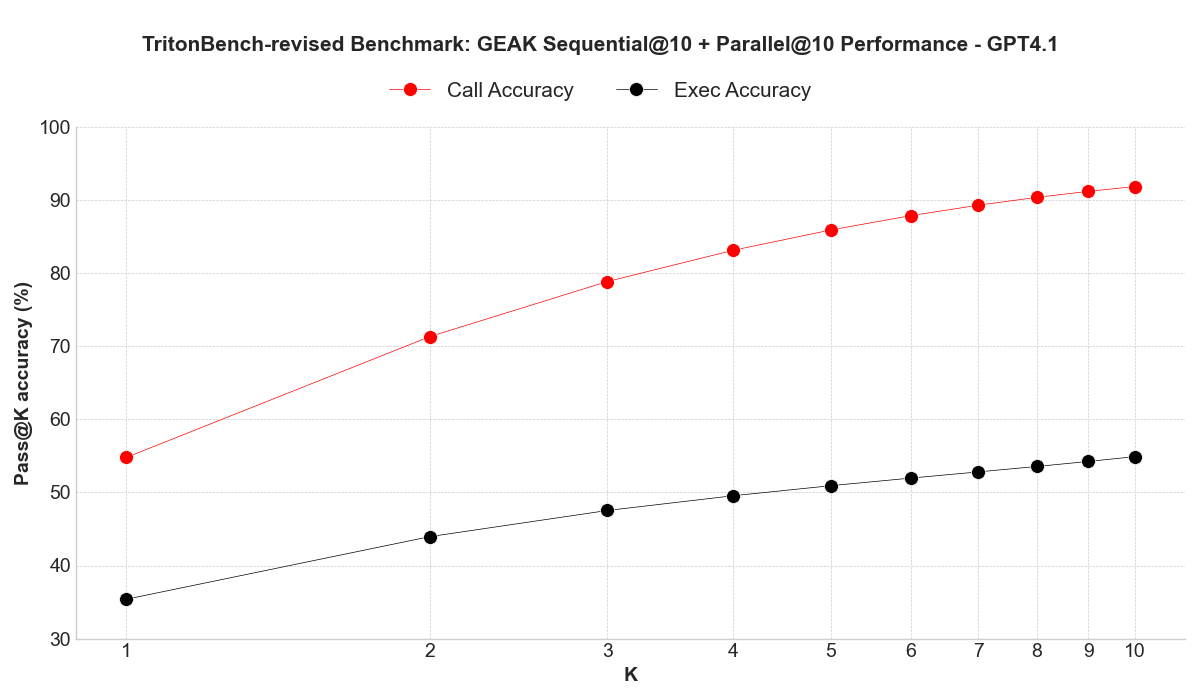
\includegraphics[width=0.85\linewidth]{figures/log_linear_tritonbench_mi300.png}
  \caption{Inference time compute scaling study on TritonBench-revised benchmark.}
  \label{fig:fig1}
\end{figure}

\begin{figure}
  \centering
  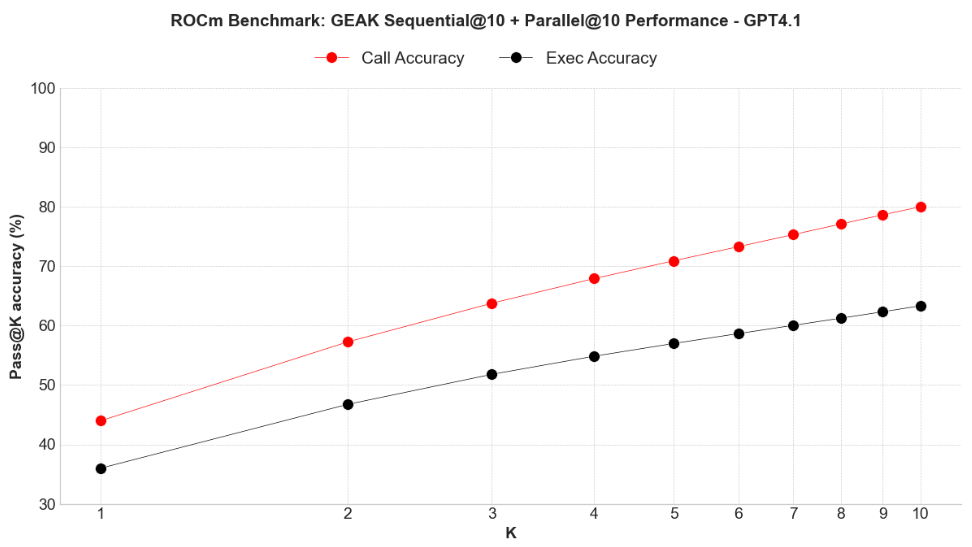
\includegraphics[width=0.85\linewidth]{figures/log_linear_rocm_mi300.png}
  \caption{Inference time compute scaling study on ROCm benchmark.}
  \label{fig:fig2}
\end{figure}

\subsubsection{Effect of different Modules}
To assess the contribution of individual components within our agent architecture, we conducted ablation experiments by evaluating performance across various combinations of modules.
Results in Table\ref{tab:modules_ablation} show that each module—knowledge injection, one-shot, and Optimizer—contributes positively to both execution accuracy and speedup, highlighting the complementary roles these components play in enhancing the agent's overall performance. 

Specifically, knowledge injection alone provides a substantial lift over the baseline, improving call accuracy from 14.67\% to 52.72\% and execution accuracy from 8.70\% to 20.11\%. This underscores the critical role of prior knowledge in enabling correct kernel generation.

Adding one-shot prompting further improves accuracy, pushing call accuracy to 54.35\% and execution accuracy to 27.17\%. However, the speedup remains under 1.0 (i.e., 0.99), suggesting that while one-shot helps with correctness, it has limited impact on runtime efficiency on its own.

The introduction of the Optimizer module shows the most significant impact on speedup. When combined with the other two modules, it boosts execution accuracy to 40.76\% and yields a notable speedup of 1.45×, the highest among all configurations. This indicates that the Optimizer not only improves the likelihood of generating correct kernels but also helps produce more efficient code in terms of latency and performance.
\begin{table}
 \caption{Modules}
  \centering
  \begin{tabular}{llllll}
    \toprule
    Knowledge Injection & 1-shot & Optimizer & call acc(\%) & exec acc(\%) & speedup \\
       \midrule
    &  &  &  14.67 & 8.70 & 0.52\\
    \checkmark & &  & 52.72 & 20.11 & 0.86 \\
    \checkmark & \checkmark & & 54.35 & 27.17 & 0.99 \\
    \checkmark & \checkmark & \checkmark & 56.52 & 40.76 & 1.45 \\
   
    \bottomrule
  \end{tabular}
  \label{tab:modules_ablation}
\end{table}


